%------------------------------------------------------------------------------
% Template file for the submission of papers to IUCr journals in LaTeX2e
% using the iucr document class
% Copyright 1999-2013 International Union of Crystallography
% Version 1.6 (28 March 2013)
%------------------------------------------------------------------------------

\documentclass[]{iucr}              % DO NOT DELETE THIS LINE
     %-------------------------------------------------------------------------
     % Information about journal to which submitted
     %-------------------------------------------------------------------------
     \journalcode{J}              % Indicate the journal to which submitted
                                  %   A - Acta Crystallographica Section A
                                  %   B - Acta Crystallographica Section B
                                  %   C - Acta Crystallographica Section C
                                  %   D - Acta Crystallographica Section D
                                  %   E - Acta Crystallographica Section E
                                  %   F - Acta Crystallographica Section F
                                  %   J - Journal of Applied Crystallography
                                  %   M - IUCrJ
                                  %   S - Journal of Synchrotron Radiation

\usepackage{verbatim}
\usepackage{graphicx}
\usepackage{tikz}
\usepackage{amsmath}
\usepackage{listings}
\usepackage{color,soul}

\lstset {
	frame=single
}
\lstdefinelanguage{ini} {
	basicstyle=\ttfamily\scriptsize,
	columns=fullflexible,
	morecomment=[s][\color{red}\bfseries]{[}{]},
	morecomment=[l]{\#},
	commentstyle=\color{blue}\ttfamily,
	morekeywords={},
	otherkeywords={=,:::},
	keywordstyle={\color{blue}\bfseries}
}

\begin{document}                  % DO NOT DELETE THIS LINE
     %-------------------------------------------------------------------------
     % The introductory (header) part of the paper
     %-------------------------------------------------------------------------

     % The title of the paper. Use \shorttitle to indicate an abbreviated title
     % for use in running heads (you will need to uncomment it).

\title{The Expand-Maximize-Compress Single Particle Imaging Algorithm}
%\shorttitle{Short Title}

     % Authors' names and addresses. Use \cauthor for the main (contact) author.
     % Use \author for all other authors. Use \aff for authors' affiliations.
     % Use lower-case letters in square brackets to link authors to their
     % affiliations; if there is only one affiliation address, remove the [a].

\author[a]{Kartik}{Ayyer}

\author[b]{Ti-Yen}{Lan}

\cauthor[c]{N. Duane}{Loh}{duaneloh@nus.edu.sg}

\author[b]{Veit}{Elser}

\aff[a]{Center for Free-Electron Laser Science, Deutsches Elektronen-Synchrotron DESY, Notkestra{\ss}e 85, 22607 Hamburg, \country{Germany}}
\aff[b]{Second affiliation address}
\aff[c]{Centre for Bio-imaging Sciences, National University of Singapore, 117543, \country{Singapore}.}

     % Use \shortauthor to indicate an abbreviated author list for use in
     % running heads (you will need to uncomment it).

%\shortauthor{Soape, Author and Doe}

     % Use \vita if required to give biographical details (for authors of
     % invited review papers only). Uncomment it.

%\vita{Author's biography}

     % Keywords (required for Journal of Synchrotron Radiation only)
     % Use the \keyword macro for each word or phrase, e.g. 
     % \keyword{X-ray diffraction}\keyword{muscle}

%\keyword{keyword}

     % PDB and NDB reference codes for structures referenced in the article and
     % deposited with the Protein Data Bank and Nucleic Acids Database (Acta
     % Crystallographica Section D). Repeat for each separate structure e.g
     % \PDBref[dethiobiotin synthetase]{1byi} \NDBref[d(G$_4$CGC$_4$)]{ad0002}

%\PDBref[optional name]{refcode}
%\NDBref[optional name]{refcode}

\maketitle                        % DO NOT DELETE THIS LINE

\begin{synopsis}
Supply a synopsis of the paper for inclusion in the Table of Contents.
\end{synopsis}

\begin{abstract}
TODO: Abstract goes here.
\end{abstract}


     %-------------------------------------------------------------------------
     % The main body of the paper
     %-------------------------------------------------------------------------
     % Now enter the text of the document in multiple \section's, \subsection's
     % and \subsubsection's as required.

\section{Introduction}
TODO: Some mumbo jumbo about how SPI will revolutionize the world.

The goal of single-particle imaging (SPI) is to assemble the three-dimensional (3D) structure of an object from incomplete data collected from very many of its copies. With X-ray Free-electron Laser (XFEL) based SPI, noisy and un-oriented two-dimensional (2D) diffraction patterns of many individual copies of the object are computationally assembled into a 3D diffraction volume. The object's 3D electron density distribution is then recovered from this diffraction volume via de novo phase-retrieval. 

TODO: Include references that discusses XFEL SPI.

\subsection{Purpose of this software package}
What is EMC? Reference 1D and 3D EMC paper. Expectation maximization in the space of unknown orientations?
Features are shot-noise-limited diffraction patterns.
How does EMC compare with other methods?
Extensions of this algorithm have been successfully adapted for tomography and crystallography [...]. Describe what is different about these applications. 

\section{Structure of this package}\label{sec:package}

This software package uses the EMC algorithm to reconstruct a 3D diffraction volume from noisy, randomly-oriented single particle diffraction patterns. These patterns could be from simulations or actual single-particle experiments.


\subsection{Typical experiment and key parameters}\label{sec:expParams}

The key parameters of the experiment are illustrated in Figure \ref{fig:expGeometry}, which include the photon wavelength $\lambda$, and the maximum scattering angle. These parameters help determine the maximum half period resolution $a$ as well as the field of view $L$ of the reconstructed electron density map. Given these parameters, one can then decide if an candidate scatterer can yield enough diffraction signal to the desired resolution. These parameters are revisited in Section \ref{subsubsec:config}.

Throughout this document, we adopt the crystallographer's convention for spatial frequency 
\begin{equation}
\widehat{q} = \frac{2 \sin(\phi_{\text{max}}\,/\,2)}{\lambda}\;,
\end{equation}
where the $\phi_{\text{max}}$ is the maximum scattering angle. We also note that a corrective factor is also needed to compensate for different solid angles subtended by different pixels on the detector (Appendix \ref{sec:solidAngle}). 

\begin{figure}
\caption{Experimental geometry of single-particle imaging adopted in the data stream simulator. This simulator implements a planar square detector comprising $d\times d$ square pixels, each of area $l_D^2$. The detector is positioned a $z_D$ from the x-ray interaction region, where the scatterer (depicted here as a sphere of radius $R_p$) is typically an electron density map sampled from a Protein Data Bank file. The incident photon wavelength is $\lambda \,\AA$. From these, one can compute the maximum scattering angle captured by the detector, subtended by gray triangles to either the edge or corner of the detector. From the former we compute the half-period resolution $a$, which is equivalent to the length of the voxel (red) in the reconstructed electron density map.}
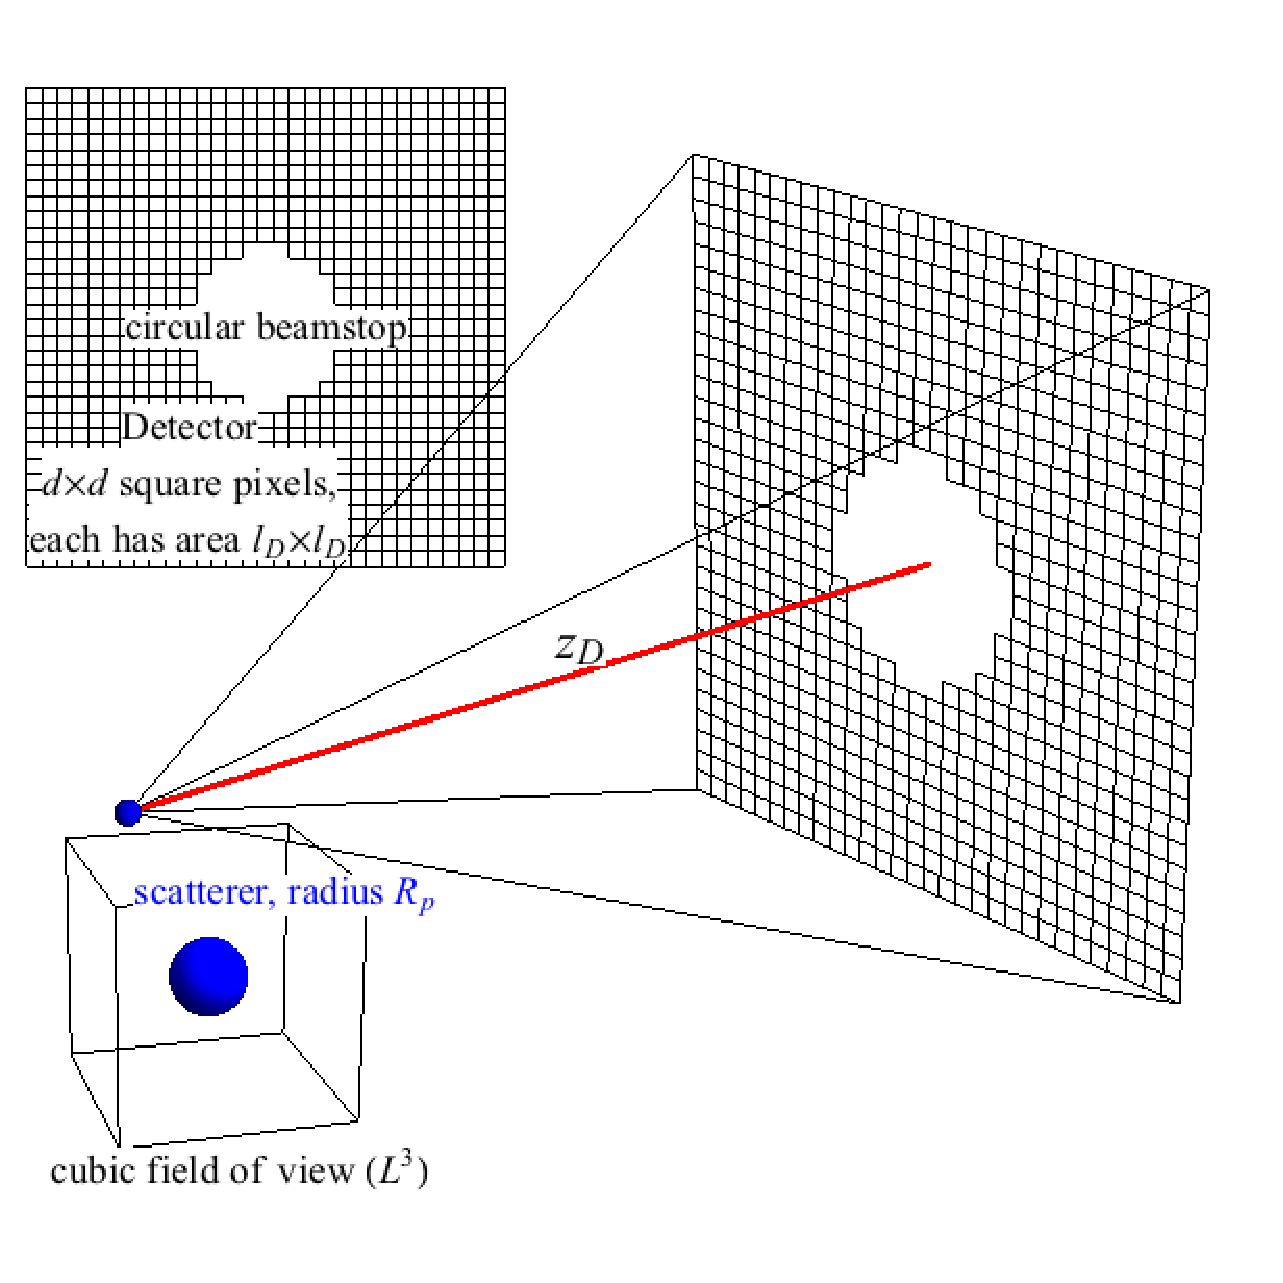
\includegraphics[width=3.5in]{figures/geometry.eps} \label{fig:expGeometry}
\end{figure}

\subsection{Data stream simulator}\label{sec:dataStreamSim}

Whether the photon patterns are derived from simulations (Figure \ref{fig:simFlowchart}) or experiments (Figure \ref{fig:expFlowchart}), the minimum input to this reconstruction package are: a configuration file, a file with detector coordinates and pixel status, and a sparse representation of the photon data from diffraction patterns. 

\begin{figure}
\caption{Flowchart of how to simulate a data set and perform a reconstruction starting from a sample PDB file and a configuration file with information about the experimental setup.}\label{fig:simFlowchart}
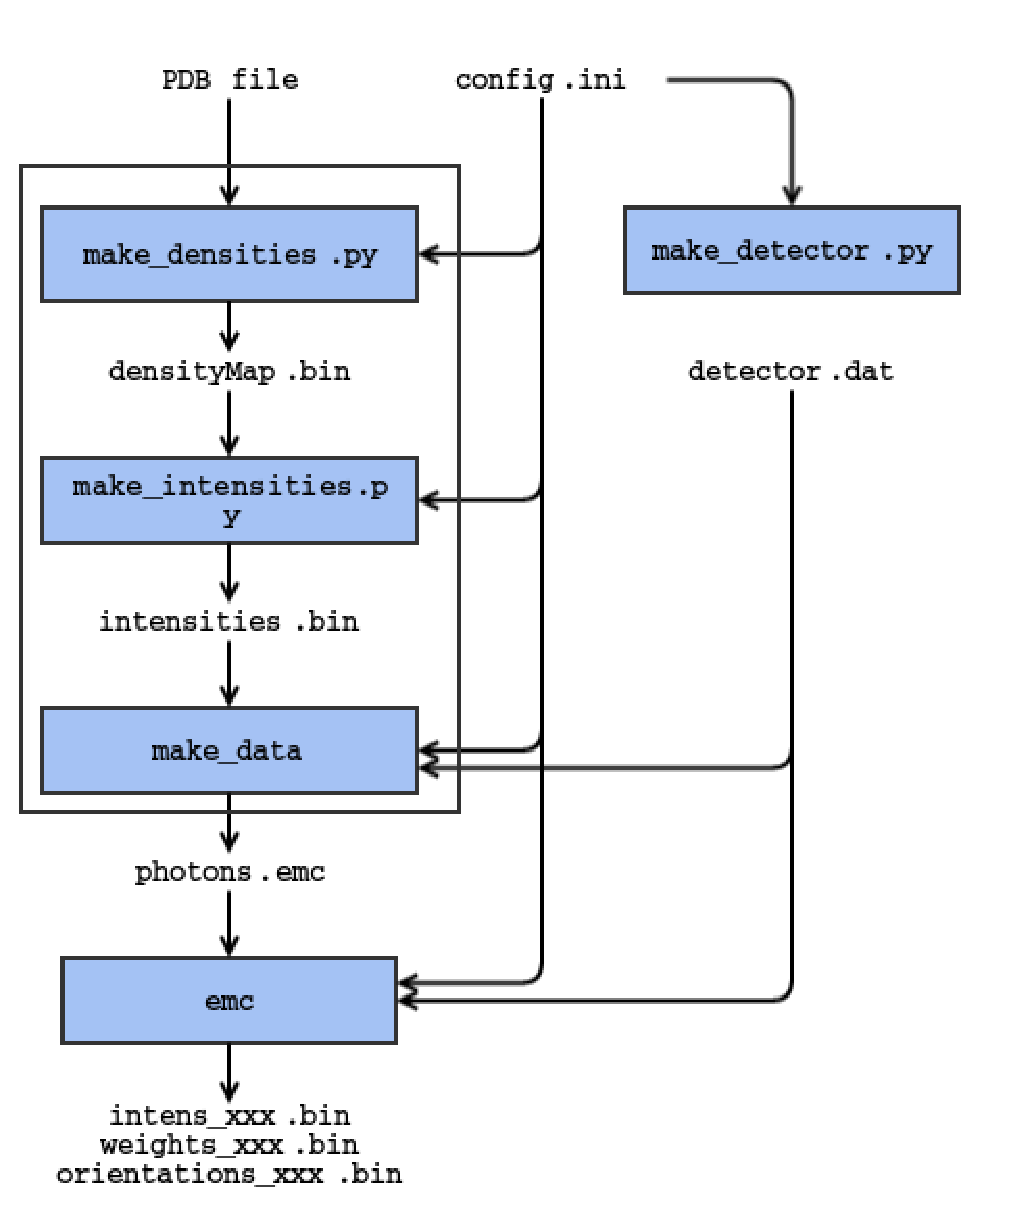
\includegraphics[width=\textwidth]{figures/emc_sim.pdf}
\end{figure}

\begin{figure}
\caption{Flowchart of how to process experimental data in sparse format. Information about the experimental parameters is placed in the configuration file and the detector geometry is in the detector file. The formats of all three input files is described in Section~\ref{subsec:formats}.}\label{fig:expFlowchart}
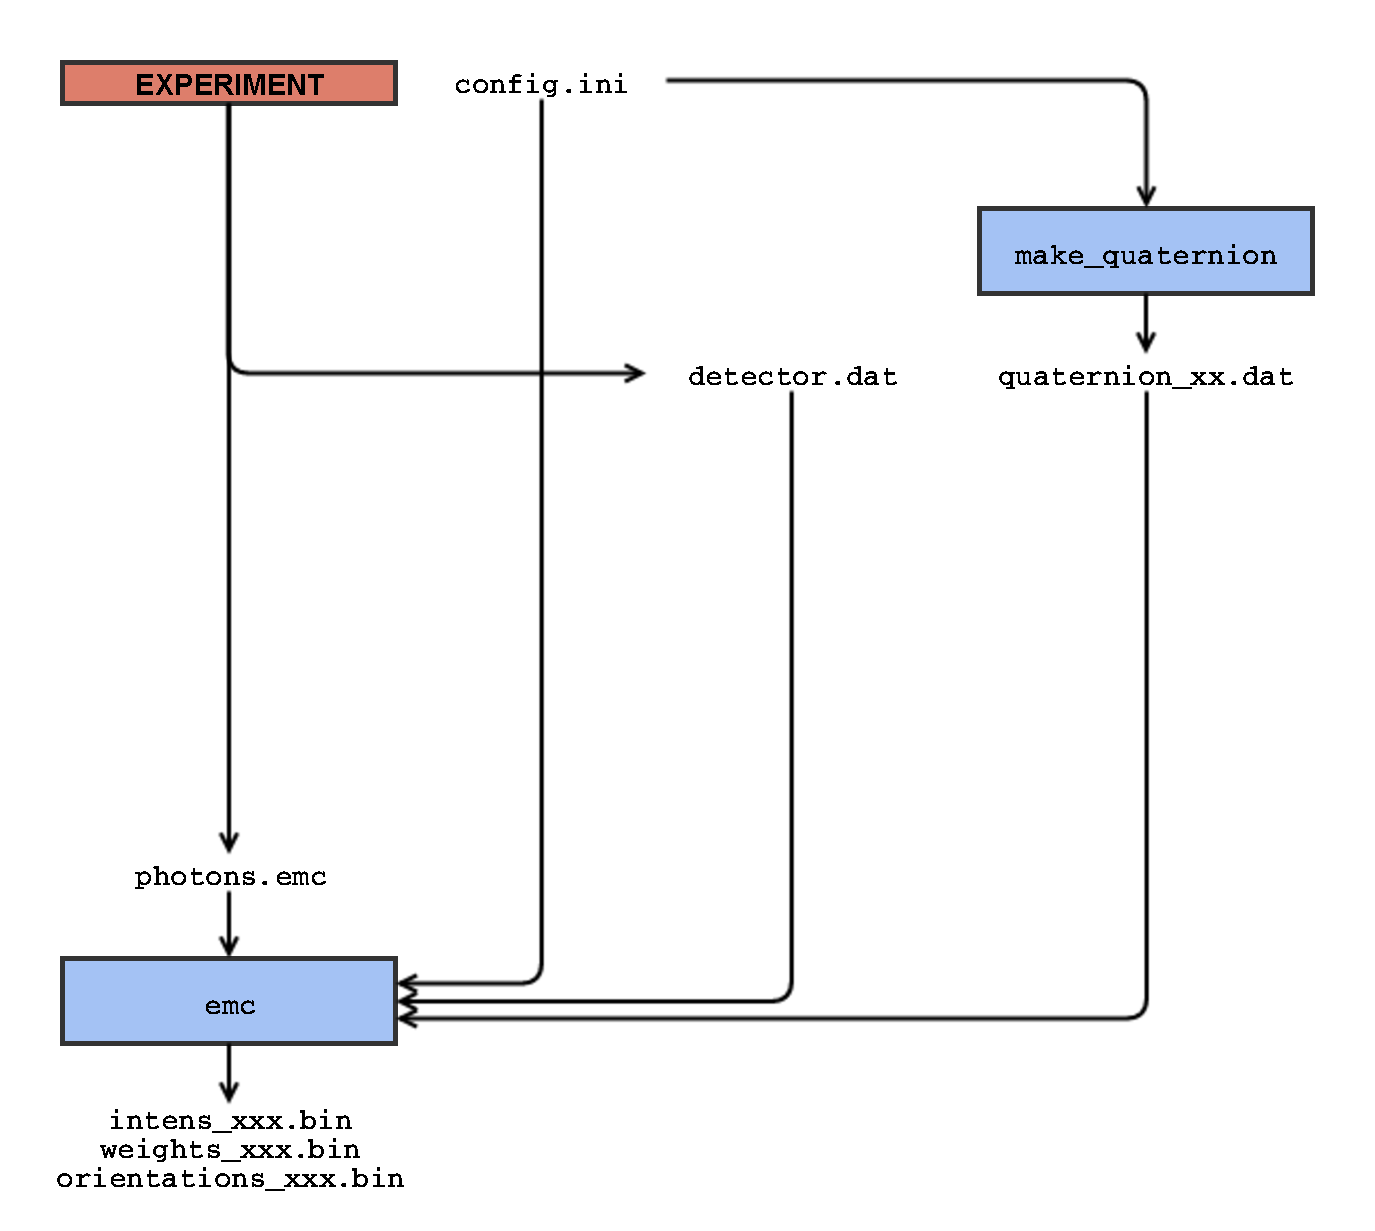
\includegraphics[width=\textwidth]{figures/emc_exp.pdf}
\end{figure}

\subsection{Implementing the EMC algorithm}\label{subsec:EMC}
The EMC algorithm \cite{loh2009} is implemented here with hybrid MPI+OpenMP, and hence suitable for shared and/or distributed memory systems. In this section, we describe this implementation and an extension to deal with high signal data. In the current version, the code assumes a Poisson probability model for the number of photons in a pixel. This means that if the mean number of photons at a pixel is $W$, the probability of getting $K$ photons is given by
\begin{equation}
P(K{\big\vert}W) = \frac{W^K e^{-W}}{K!}
\end{equation}
Gaussian noise models have been used in situations with bright, but noisy data \cite{loh2010,ekeberg2015}, but if single photons can be accurately counted, the noise model will be Poissonian. Let the number of photons at pixel number $t$ in data frame (interchangeably termed {\it photon/diffraction pattern}) $d$ be $K_{dt}$. Also let, for a given orientation $r$, the predicted mean intensity at the same pixel be $W_{rt}$. Since an independent Poisson process occurs at each pixel, the probability of that frame being generated by that particular tomogram is
\begin{equation}
R_{dr} = \prod_t \frac{W_{rt}^{K_{dt}} e^{-W_{rt}}}{K_{dt}!}
\label{eqn:probnumr}
\end{equation}
But since the particle must have some orientation, the probability of frame $d$ having orientation $r$ is obtained by normalizing over all orientations.
\begin{equation}
P_{dr} = \frac{R_{dr}}{\sum\limits_r R_{dr}}
\label{eqn:prob}
\end{equation}
With these probabilities, one can define a total log-likelihood of the data being generated by the model with the current probabilities as
\begin{equation}
Q(W') = \sum_d \sum_r \sum_t P_{dr} (K_{dt} \log(W'_{rt}) - W'_{rt})
\label{eqn:totalq}
\end{equation}
From this, we get the update rule on the tomograms $W_{rt}$ which maximize $Q$,
\begin{equation}
W'_{rt} = \frac{\sum\limits_d P_{dr} K_{dt}}{\sum\limits_d P_{dr}}
\label{eqn:wupdate}
\end{equation}

The most time-consuming step of each iteration is the calculation of Eq.~\ref{eqn:probnumr}. This involves comparing all the tomograms with all the patterns for each pixel which has at least one photon. The code is parallelized over orientations, so each MPI and OpenMP rank performs the calculation for a subset of orientations. At the start of the iterations, each MPI rank gets a copy of the current 3D intensity model. Each MPI and OpenMP rank then calculate the relevant tomograms, $W_{rt}$, on the fly and calculate $R_{dr}$ for that orientation using Eq.~\ref{eqn:probnumr}. In order to perform the normalization operation of Eq.~\ref{eqn:prob}, reduction operations across all ranks. The $P_{dr}$ array is then used to calculate updated tomograms for each $r$, and then merged to obtain an updated 3D model for each MPI rank. These models are then reduced to obtain the final updated model.

In many experimental situations, the incident fluence varies from shot-to-shot. Thus, the tomograms would be scaled differently for each pattern. One can enable the recovery of these scale factors using the update rule described in Appendix~\ref{sec:rescaling}. 

We also find that if the signal is too strong, the reconstructions get stuck in local maxima by having all the orientations overlap each other. This effect is similar to what is observed if the background is too high~\cite{ayyer2015}. However, we also observe that the reconstruction is stable around the true solution, and only falters when one starts from a random initial guess. This problem can be avoided by using the deterministic annealing variant of expectation maximization ~\cite{ueda1998}. In the EMC case, this is implemented by raising $R_{dr}$ calculated in Eq.~\ref{eqn:probnumr} to a small power $\beta$, and then normalizing. This has the effect of broadening the distribution and results in a rotationally blurred, but stable reconstruction. The power $\beta$ can then be raised gradually in a manner similar to simulated annealing to slowly improve the reconstruction. An example of this is shown in Section~\ref{subsec:recon}, where $\beta$ starts at 0.001 and is raised by a factor of 2 every 10 iterations 8 times.

\subsection{Modules and convenience utilities}\label{subsec:mod+utils}
\subsubsection{Modules}\label{subsubsec:mods}
Here are the essential modules for simulating a data stream from a single-particle imaging experiment. By default, these modules uses parameters listed in a single \texttt{config.ini} configuration file, although point each module to different configuration files for each is straightforward as well.

\begin{enumerate}
\item{\bf make\_detector.py.} Creates a detector file using the experimental parameters specified in the configuration file. The format of this file is specified in Section~\ref{subsubsec:detector}.
\item{\bf make\_densities.py.} Creates an electron density map from a PDB file, given the resolution and field of view expected from the configuration file.
\item{\bf make\_intensities.py}. Creates a set of 3D diffraction intensities from an electron density map and the experimental parameters found in the configuration file.  
\item{\bf make\_data}. Simulates a sparse photon diffraction pattern using a 3D diffraction volume (e.g. the one generated by {\bf make\_intensities.py}), and the configuration file. By default these photon data are saved as a binary file, \texttt{photons.emc}, detailed in Section~\ref{subsubsec:emcformat}.
\item{\bf make\_quaternion}. Creates a list of quasi-uniform rotation group samples based on a refinement scheme of the 600-cell, as described in \citeasnoun{loh2009}. These samples are used by the {\bf emc} reconstruction algorithm, as instructed by the \texttt{config.ini} configuration file.
\end{enumerate}

\subsubsection{Convenience utilities}\label{subsubsec:utils}
Several convenience utilities are included to help prepare the data for or view the results from the EMC reconstruction algorithm. These utilities are briefly described here. 
\begin{enumerate}
\item{\bf init\_new\_recon.py.} This Python utility compiles the C executables in the package, and makes them plus other the rest of the utilities available in a newly initialized reconstruction sub-directory.
\item{\bf sim\_setup.py.} This Python utility simulates a single-particle data stream using the parameters listed in the configuration file. This utility, in turn, calls the following modules listed above: {\bf make\_densities.py}, {\bf make\_intensities.py}, {\bf make\_data.py}, and {\bf make\_quaternions.py}.
\item{\bf make\_powder.py}. Makes a virtual powder pattern from a large stack of diffraction patterns stored in the sparse photon format adopted in this package.
\item{\bf run\_emc.py}. Starts the EMC reconstruction by calling its MPI+OpenMP implementation in C. Includes a few convenience operations like calling the {\bf make\_quaternion} module to increase the sampling of the rotation group just before starting a reconstruction.
\item{\bf autoplot.py}. Renders the results of the EMC reconstruction, including the diagnostics it generates, with the option of automatically updating the plots when newer intensities become available.
\end{enumerate}


\subsection{Configuration and data formats}\label{subsec:formats}
\subsubsection{Configuration file}\label{subsubsec:config}
The configuration file is used to pass parameters and file names to the main reconstruction code as well as to the various utilities. The file has the standard \texttt{key = value} format with the parameters for different modules grouped by module names in square brackets. There is a global \texttt{[parameters]} section containing information about the experimental setup. A typical configuration file is shown in Fig.~\ref{fig:config}, which corresponds to the first simulation case in Table \ref{table:simParams}. This default file also shows the use of special keywords used to point to other configuration file parameters (eg. \texttt{in\_photons\_file}). The \texttt{[parameters]} section is described below. For other sections, refer to the appropriate module in Section~\ref{subsec:mod+utils}.

The basic parameters of the experiment are:
\begin{itemize}
\item \texttt{detd}: Detector distance in mm
\item \texttt{lambda}: Wavelength in \AA
\item \texttt{detsize}: Detector size (assuming square detector) in pixels
\item \texttt{pixsize}: Pixel size in mm
\item \texttt{stoprad}: Radius of beamstop in pixels
\item \texttt{polarization}: Polarization direction (can be x, y, or none)
\end{itemize}

\begin{figure}
\begin{lstlisting}[language=ini]
[parameters]
detd = 300
lambda = 6.2
detsize = 150
pixsize = 0.512
stoprad = 10
polarization = x

[make_densities]
in_pdb_file = aux/4BED.pdb
scatt_dir = aux/henke_table
out_density_file = data/densityMap.bin

[make_intensities]
in_density_file = make_densities:::out_density_file
out_intensity_file = data/intensities.bin

[make_detector]
out_detector_file = data/det_sim.dat

[make_data]
num_data = 300000
fluence = 1e10
in_detector_file = make_detector:::out_detector_file
in_intensity_file = make_intensities:::out_intensity_file
out_photons_file = data/photons.emc

[make_quaternion]
num_div = 9
out_quat_file = aux/quat_09.dat

[emc]
in_photons_file = make_data:::out_photons_file
in_detector_file = make_detector:::out_detector_file
in_quat_file = make_quaternion:::out_quat_file
out_folder = data/
log_file = EMC.log
need_scaling = 0
alpha = 0.
beta = 1.
\end{lstlisting}
\caption{Typical configuration file describing various parameters used to perform a basic simulation and reconstruction using the KLH1 (\texttt{4BED.pdb}) molecule. Compare these with numbers from Table \ref{table:simParams}.}
\label{fig:config}
\end{figure}

\subsubsection{Detector file}\label{subsubsec:detector}
The detector file is an ASCII (human readable) file which describes various properties of the detector. The first line of the file contains a single number which represents the number of pixels. Following that, for each pixel, there are five columns of numbers. The first three columns give the 3D coordinates of the detector pixel in voxels, where the voxels refer to the 3D grid containing the intensity model. The next column gives the product of the polarization and solid angle corrections for that pixel. The last column is an 8-byte unsigned integer whose value is used by the EMC code as well as other utilities to categorize the pixel. Currently, there are three categories:
\begin{itemize}
\item 0: Good pixel, used to determine the orientation of a given pattern.
\item 1: These pixels will not be used to determine the orientation, but will still be merged into the 3D grid using the orientations calculated from category 0 pixels.
\item 2: Bad pixel. Pixels whose value will be used neither to determine the orientation nor to calculate the merged 3D intensities.
\end{itemize}

\subsubsection{Photons file (emc format)}\label{subsubsec:emcformat}
Since the data in many relevant experiments utilizing the EMC algorithm have very few photons/pattern, a sparse binary format is used to store the data. Instead of storing the number of counts at each pixel, only the locations of non-zero counts are stored. since most of the non-zero counts are ones, only the locations of those are stored. For the rest, two numbers are stored, the location and photon count. 

The header resides in the first 1024 bytes. The first 4 bytes are a 32 bit integer giving the number of patterns (\texttt{num\_data}) contained in the file. The next 4 bytes are also a 32 bit integer giving the number of pixels in the detector file used to number the pixels. The next 1016 bytes are currently empty (filled with zeros).

After this, there are \texttt{num\_data} 32 bit integers giving the number of one-photon events in each pattern (\texttt{ones}). Similarily, there are \texttt{num\_data} integers giving the number of multi-photon events (\texttt{multi}). The total number of single photon events in all the patterns is the sum of all numbers in the \texttt{ones} array ($S_o$). Similarily, let $S_m$ be the total number of multiple photon events. The file contains $S_o$ 32 bit integers giving the locations of the single photon pixels, and then $S_m$ integers with the locations of the multiple photon pixels. This is followed by $S_m$ integers giving the number of photons in each of those multiple photon pixels. 

\section{Example reconstructions of simulated experiments}\label{sec:simulations}

We exemplify our package with three simulated single-particle reconstructions using the specifications of Atomic Molecular and Optical Science (AMO)~\cite{ferguson2015} and Coherent X-ray Imaging (CXI) ~\cite{liang2015} endstations at Linac Coherent Light Source (LCLS) \cite{Emma2010}. For these experiments chose to simulate the reconstruction of keyhole limpet hemocyanin \hl{(KLH) 1 didecamer}~\cite{gatsogiannis2009} and four-layer Tobacco Mosaic Virus (TMV)~\cite{bhyravbhatla1998} at AMO and CXI respectively. Notably, the choices in Table \ref{table:simParams} yield and average of $\sim 100$ photons per single-particle diffraction pattern.

\begin{table}
\caption{Parameters for EMC reconstructions of simulated single-particle imaging.} \label{table:simParams}
\label{parameters}
\begin{tabular}{p{3.5cm} p{1.4cm} p{1.4cm} p{1.4cm}}
                        			& AMO (low)          & CXI              & AMO (high)\\
\hline
photon energy (keV)     	& 2.0                 & 7.0              & 2.0 \\
$\lambda$, photon wavelength (\AA)	& 6.2                 & 1.77             & 6.2 \\
$z_D$, detector distance (mm)  	& 300                 & 350              & 290 \\
$d$, detector size (pixel)   	& 150                 & 150              & 150 \\
$l_D$, pixel side length (mm)         		& 0.512               & 0.751            & 0.512 \\
$L$, full field of view (nm) 	& 363		& 82.4		& 351 \\
beamstop radius (pixel) 	& 10.0                & 8.0              & 10.0 \\
fluence (photons/um$^2$)& $1\times10^{10}$\footnote{Estimated from \citeasnoun{Loh2013}.}    & $1\times10^{12}$ & $\mathbf{3.1\times10^{12}}$ \\
$a$, half-period resolution\footnote{Resolution defined from detector's edge.}(nm) 	& 2.45                & 0.56             & 2.5 \\
\hline
particle                  		& KLH1\footnote{Keyhole Limpet Hemocyanin 1. \label{KLH1}}& TMV\footnote{Four-layer Tobacco Mosaic Virus.}& KLH1$^\ref{KLH1}$ \\
mass (kDa)	            	& 8000                & 18               & 8000 \\
$R_p$, particle radius (nm) 		& 18.9                & 9.3                & 18.9 \\
$\widetilde{R}$\footnote{Dimensionless radius, $R_p / a$.}, dimensionless radius  & 7.7               & 16.6               & 7.6 \\
$\sigma$, speckle sampling\footnote{Defined as $\widetilde{R} = L\,/(2 R_p)$. See appendix \ref{sec:speckle}.}  & 9.6                & 4.45               & 9.2 \\
$N$, mean photons/frame & 90                  & 90               &  $\mathbf{2.8\times10^{4}}$ \\
number of data frames & $3\times 10^5$       & $5\times 10^5$    & $1\times 10^5$ \\
max. quaternion sampling\footnote{Sampling and criterion defined in \citeasnoun{loh2009}.}   & 9                   & 16                & \hl{9} \\

\end{tabular}
\end{table}

The simulation parameters are shown in Table \ref{parameters}. The detectors here had $1024\times1024$-pixels, taking on the pixel pitch of the pnCCD\cite{Struder2010} and CSPAD\cite{hart2012} detectors. We decrease the beam fluence to obtain mean photon counts $N\sim 90$ for the first two simulations, mimicking realistic losses from imperfect beam transmission, optics, and cleanup apertures \cite{Loh2013}. 

For data sufficiency we use the signal-to-noise ratio parameter defined in Eq. 37 of \citeasnoun{loh2009}, 
\begin{equation}
S = \sqrt{\frac{N M_{data}}{M_{rot}}}\; ,
\end{equation}
to estimate the required number of data frames $M_{data}$ for $S\sim50$, where $M_{rot}$ is the number of rotation samplings. Assuming the diffraction patterns are uniformly distributed in orientation space, $S^2$ can be interpreted as the average number of photons per orientation.

The third simulation of of Table \ref{table:simParams} was designed to demonstrate how deterministic annealing method can deal with convergence issues caused by very high signal. Most of the parameters were kept identical to the low fluence AMO simulation, but the fluence was up-adjusted to receive 1 mJ x-ray pulses (within an order of magnitude of design specifications \cite{Emma2010}).

\subsection{Discussions on simulated reconstructions} \label{subsec:recon}
Figures \ref{fig:amo_low_intens}, \ref{fig:cxi_intens} and \ref{fig:amo_high_intens} show orthogonal slices through the final converged intensities for the three parameter sets mentioned above. Accompanying each figure is a set of plots generated by \texttt{autoplot.py} which can be used to monitor the progress of the reconstruction. We first describe Fig.~\ref{fig:amo_low_log} as it is the most straightforward one. The leftmost plot shows the root mean squared change between the 3D intensity models in successive iterations. This is, of course, the most straightforward indicator of convergence. 

In the next column, the top plot shows the average mutual information of $P_{dr}$. This is defined as
\begin{equation}
I_d(K, \Omega) = \sum_r P_{dr} \log(P_{dr} / P_{r})
\end{equation}
where $P_r$ is the prior probability of orientations (assumed to be uniform except for a small variation due to non-uniform quaternion sampling). This is a measure of the `peakiness' of the probability distribution over orientations. For a Delta function distribution, the value is the log of the number of quaternion samples. Below that is a plot of the total log-likelihood in Eq.~\ref{eqn:totalq}. In most situations, this quantity increases monotonically, and a significant decrease indicates an error. 

The rightmost plot is the most useful for monitoring convergence. This is a matrix plot where the vertical axis is the frame number while the horizontal is iteration. The color represents the orientation number of the best orientation (maximum $P_{dr}$) for each frame. The rows have been sorted by the orientation number of the last iteration. Thus, the colors at the right end form a smooth color bar. The variation of colors along a row indicates how the most likely orientation has changed for that frame. Thus, if the colors vary smoothly over a few iterations, this indicates that most likely orientations are not changing from iteration to iteration which is a good indicator of convergence.

For the CXI reconstruction (Fig.~\ref{fig:cxi_log}), due to the size of the problem, the quaternion sampling number was increased in steps. If one chooses too coarse a rotation group sampling, low resolution speckles get reconstructed but higher resolution features remain blurry. However, once the switch to the right sampling is made, convergence is very quick. As the computation time scales as the number of samples, it is faster to slowly ramp up the fineness such that only a few iterations are performed at the highest sampling rate. The red dashed lines indicate iterations where the sampling rate was increased, starting from 6 and ending at 9. Also, since the orientation numbers change when modifying the quaternion file, each subset is independently sorted in the best orientation matrix plot. Also note how the mutual information does not increase much in the last jump, indicating that even finer sampling would not help.

For the high fluence AMO reconstruction (Fig.~\ref{fig:amo_high_log}), the situation is slightly different. As mentioned before, due to very high signal, the algorithm can fall into a local maxima trap in the first few iterations. This can be avoided by choosing a low $\beta$ as described in Section~\ref{subsec:EMC} to start with. In this particular case $\beta$ was 0.001 for the first 10 iterations and was then doubled every 10 iterations. Once again, the dashed lines represent the iterations at which $\beta$ was doubled.

\begin{figure}
\caption{Convergence of diffraction speckle features in a simulated AMO single-particle experiment (parameters listed in Table \ref{table:simParams}). In each row we render central slices of the 3D diffraction intensities recovered from KLH1 during an EMC reconstruction, after iterations 1,10,20 and 50 in ascending row order. These figures were generated by the \texttt{autoplot.py} utility of Section ~\ref{subsubsec:utils}.}
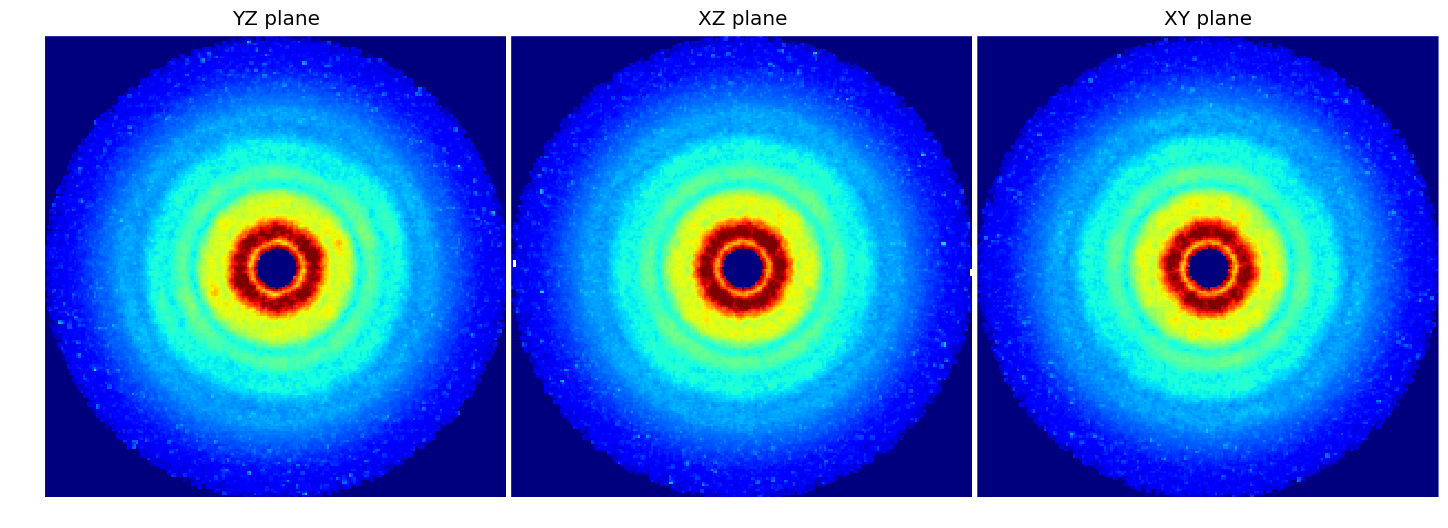
\includegraphics[width=3.5in]{figures/amo_low_intens_001.png} 
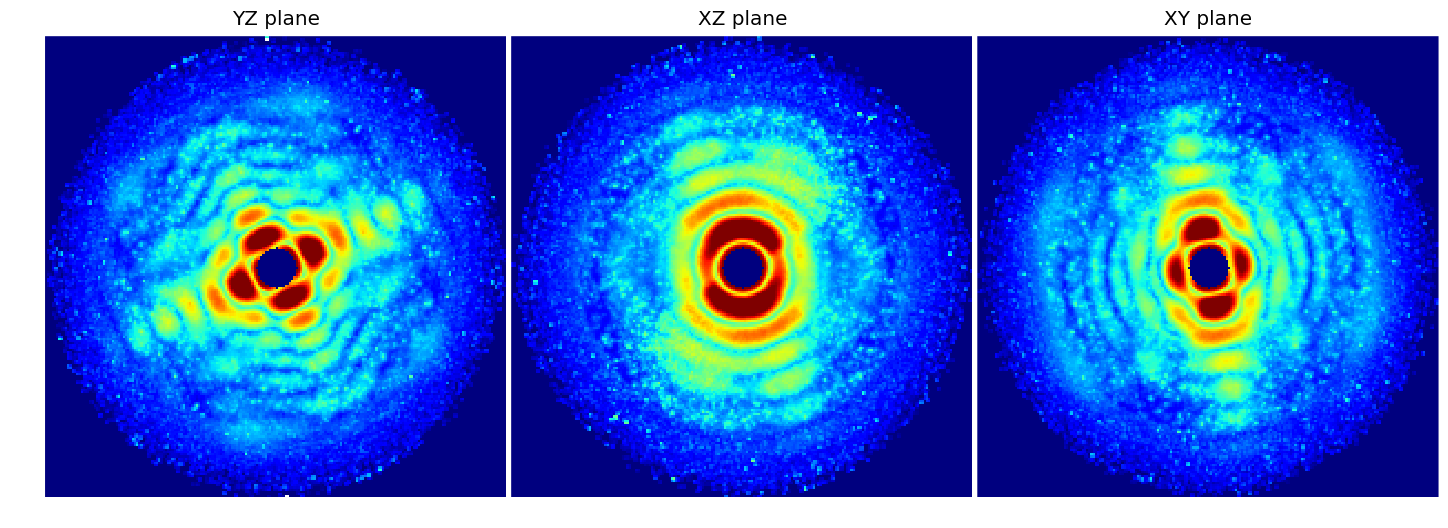
\includegraphics[width=3.5in]{figures/amo_low_intens_010.png}
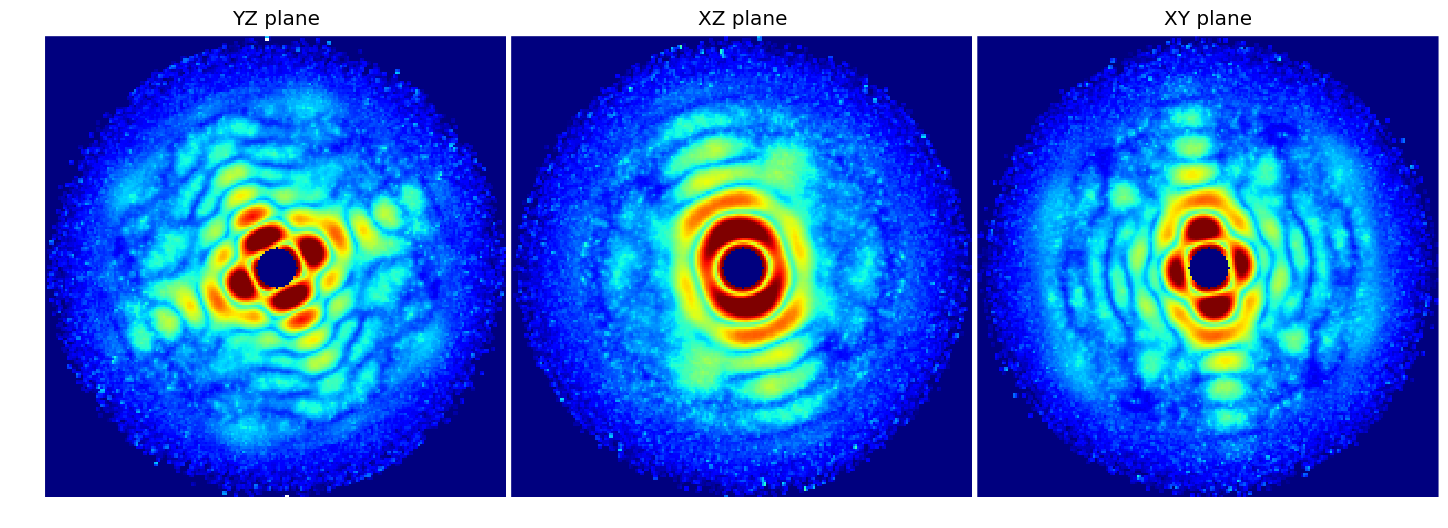
\includegraphics[width=3.5in]{figures/amo_low_intens_020.png} 
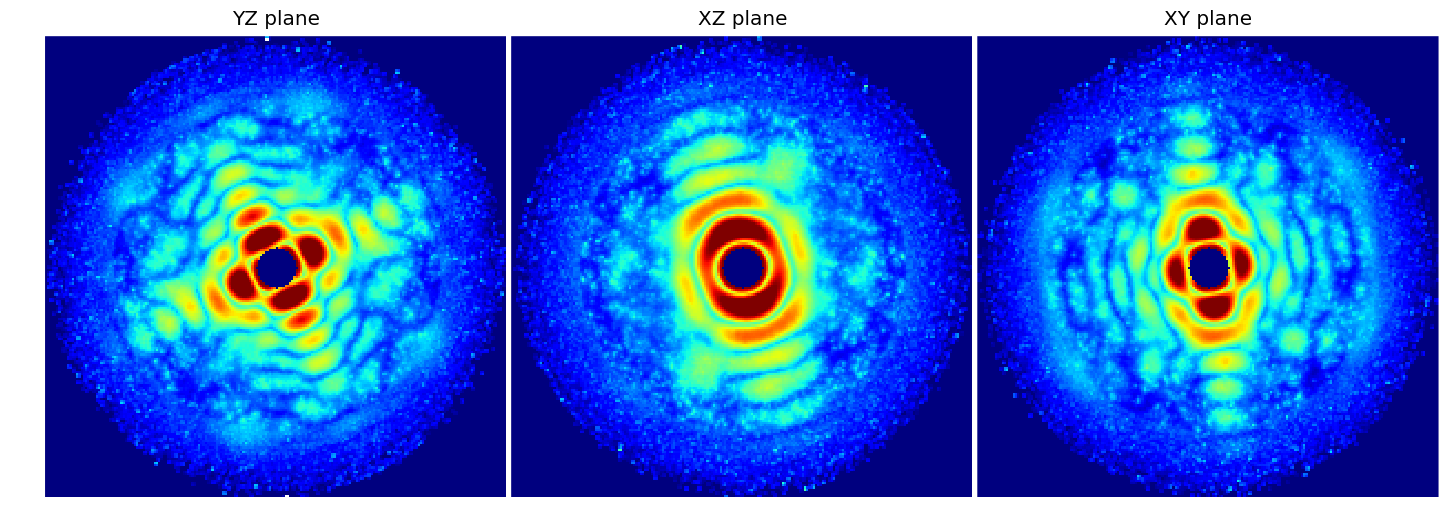
\includegraphics[width=3.5in]{figures/amo_low_intens_050.png} \label{fig:amo_low_intens}
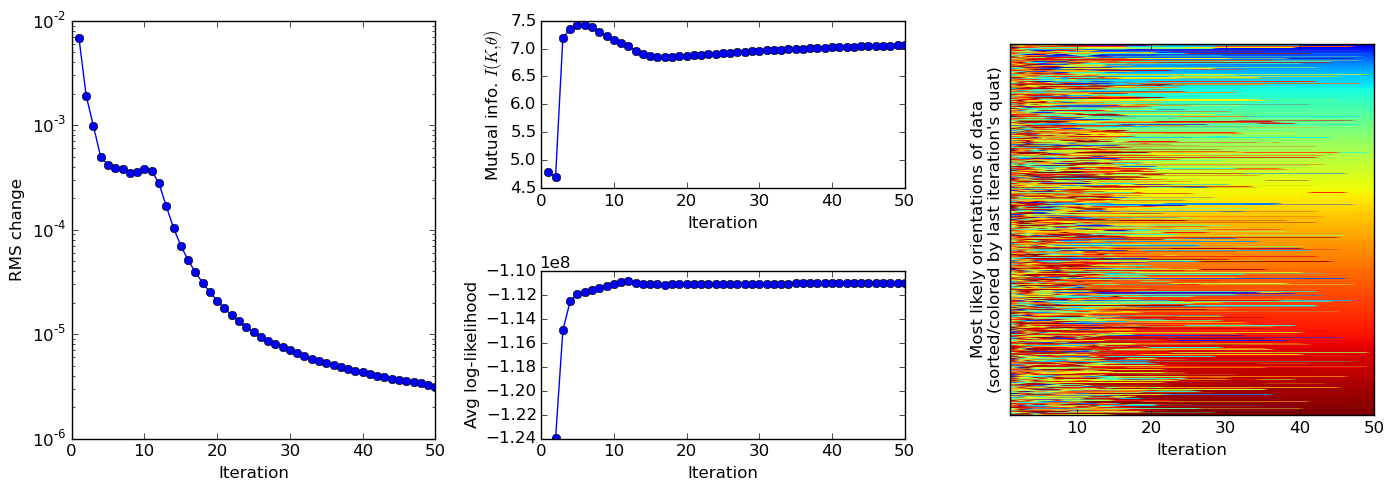
\includegraphics[width=3.5in]{figures/amo_low_log.png} \label{fig:amo_low_log}
\end{figure}

\begin{figure}
\caption{The simulated reconstruction of TMV at the CXI endstation of LCLS (see Table \ref{table:simParams}). Show here are the central sections of the reconstructed 3D diffraction volume of TMV after 55 iterations. With 88 Intel Xeon X7542 (2.67 GHz) cores this full reconstruction took 7 hours, spending 15 minutes for each of the slowest refinement iterations using 204,960 rotation group samples.}
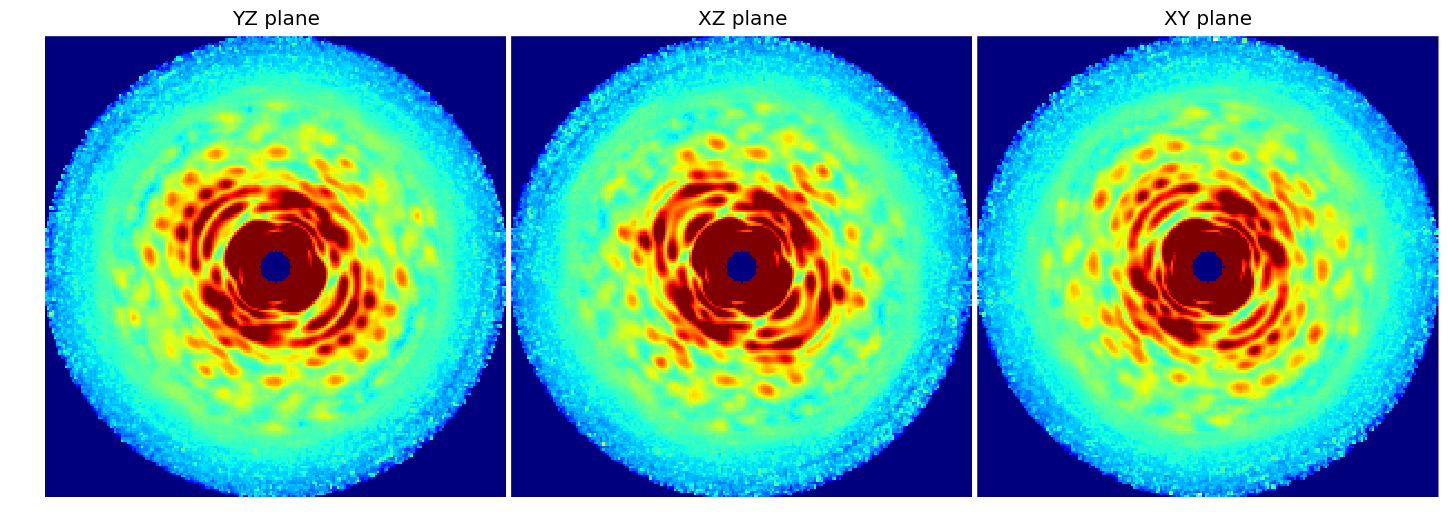
\includegraphics[width=3.5in]{figures/cxi_intens_055.png} \label{fig:cxi_intens}
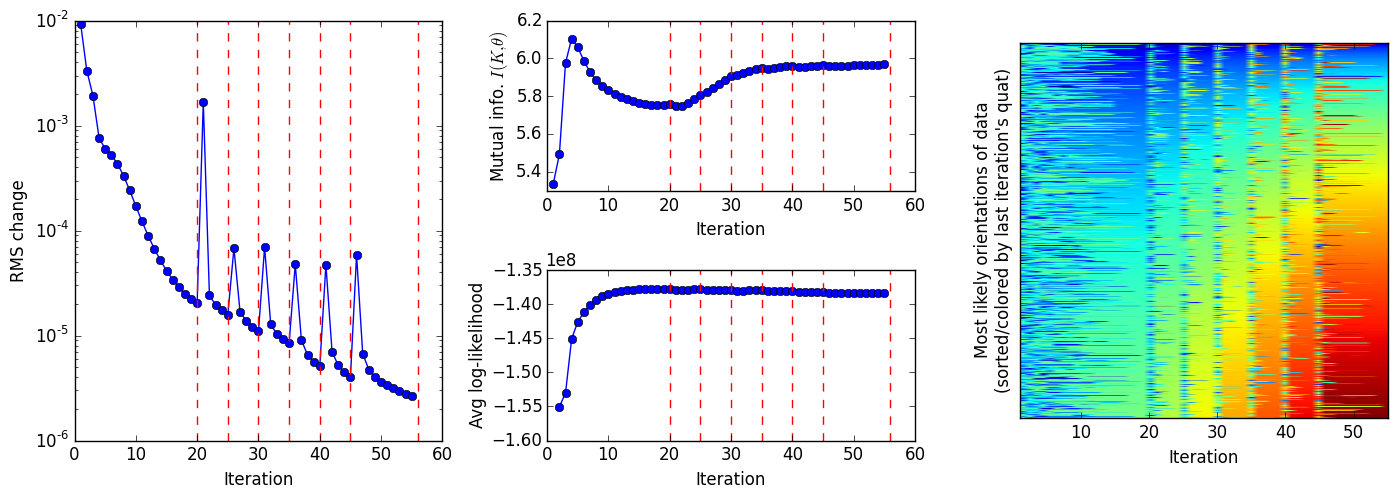
\includegraphics[width=3.5in]{figures/cxi_log_fig.png} \label{fig:cxi_log}
\end{figure}

\begin{figure}
\caption{A simulated reconstruction at the AMO endstation at LCLS with high photon fluence (see Table \ref{table:simParams}).}
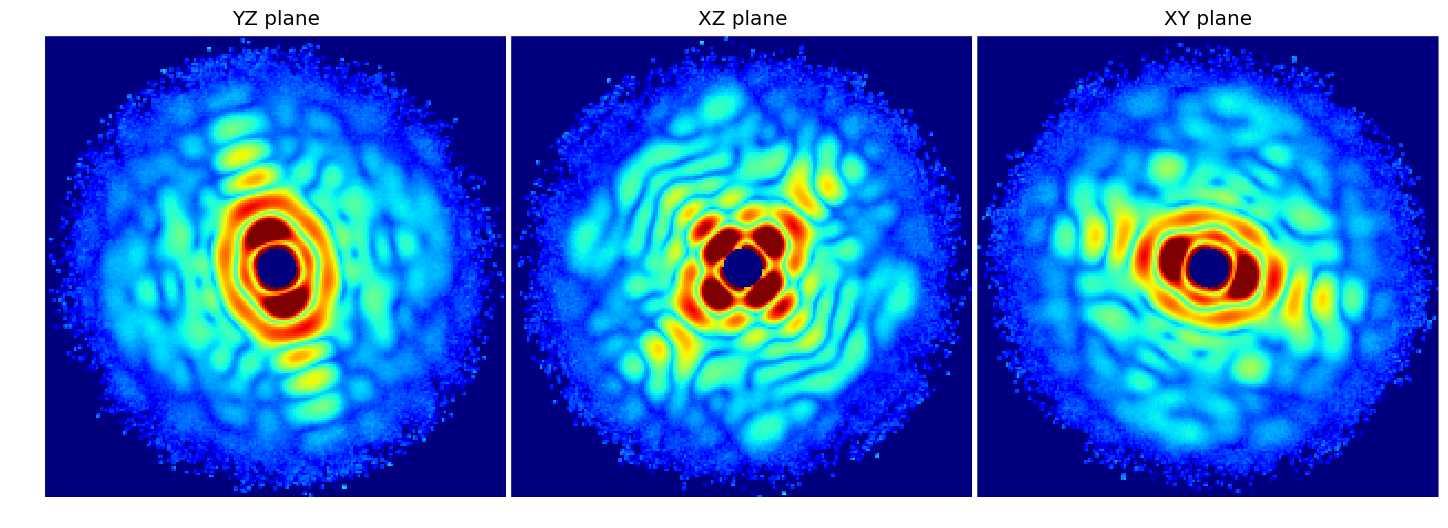
\includegraphics[width=3.5in]{figures/amo_high_intens.png} \label{fig:amo_high_intens}
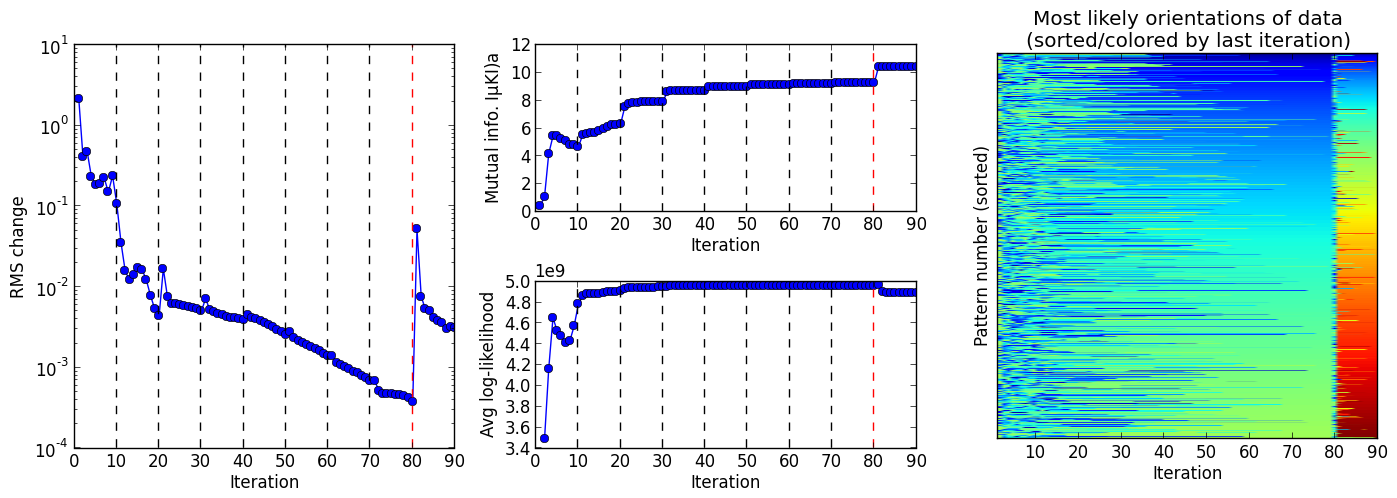
\includegraphics[width=3.5in]{figures/amo_high_log.png} \label{fig:amo_high_log}
\end{figure}


\section{Conclusions and future work}

TODO:

%%%%%%%%%%%%%%%%%%%%%%%%%%%%%%%%%%%%%%%%%%%%%%%%%%%%
%%%%%%%%%%%%%%%%%%%%%%%%%%%%%%%%%%%%%%%%%%%%%%%%%%%%

\appendix

\section{Computing speckle sampling on the detector}\label{sec:speckle}
We use a spherical approximate to estimate the size of diffraction speckles from a scatterer. A sphere of radius $R_p$, produces diffraction intensities 
\begin{equation}
I(\widetilde{q}) = \left|\frac{\sin(\widetilde{q}) - \widetilde{q} \cos(\widetilde{q})} {\widetilde{q}^3} \right|^2 \;, \label{eqn:speckle}
\end{equation}
with dimensionless resolution $\widetilde{q} = 2 \pi \widehat{q} R_p$, where we define $\widehat{q} = 2 \sin(\phi/2) / \lambda$ as the spatial resolution commonly used in structural biology. Here, $\phi$ and $\lambda$ are the scattering angles and photon wavelength respectively (see Figure \ref{fig:solidAngle}). The width of a diffraction speckle of this spherical approximate is the separation in $\Delta \widehat{q} $ between the zeros of \eqref{eqn:speckle}. These zeros occur when 
\begin{equation}
\tan(\widetilde{q}) = \widetilde{q} \;,
\end{equation}
which approaches $\widetilde{q} \to (2n+1) \pi / 2$, where $n \in \mathbb{Z}$, for large $\widetilde{q}$. As a result, for large $\widetilde{q}$ the separation between the zeros of \eqref{eqn:speckle} $\Delta \widetilde{q} \to \pi$, which results in a speckle width in spatial frequency of 
\begin{equation}
\Delta \widehat{q} \to 1/(2 R_p) \;. 
\end{equation}
Referring to Figure \ref{fig:expGeometry}, the coarsest spacings in spatial frequency occur at small scattering angles and is inversely proportional to the field of view $L$, or $\Delta \widehat{q}_{\text{min}} \sim 1/L$. 

The sampling ratio of the diffraction speckle is defined as:
\begin{equation}
\Delta \widehat{q} \,/\, \Delta \widehat{q}_{\text{min}} = \frac{L}{2R_p} = \frac{\lambda}{4 R_p \sin\left( \arctan (l_D / z_D) \,/\,2 \right)}\; ,
\end{equation}
where $l_D$ is the width of the detector pixel, and $z_D$ is separation between the detector and interaction region (see Figures \ref{fig:expGeometry} or \ref{fig:solidAngle}). While the ideal sampling ratio of the diffraction speckles should exceed two, the time and memory required for intensity reconstruction rises rapidly when this ratio becomes excessively large (e.g. $ \Delta \widehat{q} \,/\, \Delta \widehat{q}_{\text{min}} \gg 5$). 

\section{Solid angle correction for square pixels on planar detectors}\label{sec:solidAngle}
\begin{figure}
\caption{Setup for solid angle correction. In this section we compute the solid angle subtended by the square pixel (red) on the detector plane (gray). The scatterer (blue sphere) is set at the origin of this figure.}
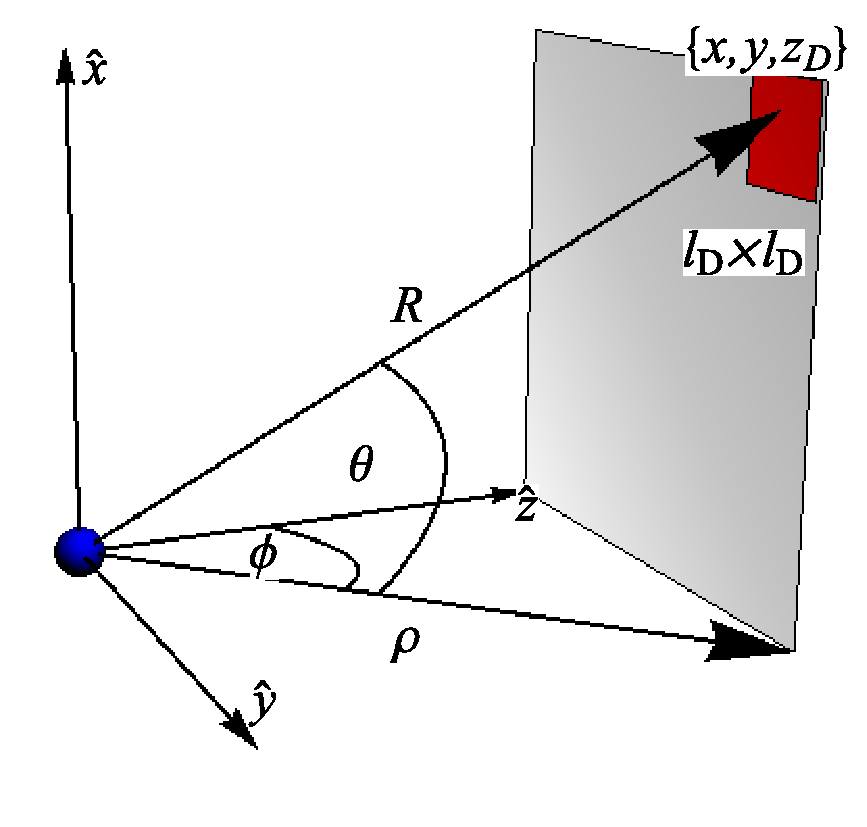
\includegraphics[width=2.5in]{figures/solidAngle.eps} \label{fig:solidAngle}
\end{figure}


In this section we compute the solid angle $\Delta \Omega$ subtended by a square pixel of area $l_D \times l_D$ about the point where a scatterer sits (see Figure \ref{fig:solidAngle}). To first approximation, the solid angle $\Delta \Omega \sim \cos(\theta) \Delta \phi \cdot \Delta \theta$. The estimate  $\Delta \phi$ and $\Delta \theta$, we use the following relations. On a detector $z_D$ from the interaction point, we consider a pixel at position $\{x,y,z_D\}$ in its spherical coordinate representation:
\begin{equation}
\sin (\phi) = y /\rho ,&\qquad \cos(\phi) = z_D / \rho \;,
\end{equation}
where $\rho = \sqrt{y^2 + z_D^2}$.
Differentiating $\sin(\phi)$ with respect to $\phi$ gives
\begin{equation}
\cos(\phi) \Delta \phi \approx \frac{\Delta y}{\rho} \left[1 - \left( y/\rho\right)^2 \right]\;.
\end{equation}
Repeating this for $\theta$
\begin{equation}
\sin (\theta) = x /R ,\;  \cos(\theta) = \rho / R \;,
\end{equation}
with $R = \sqrt{x^2 + y^2 + z_D^2}$, leads to 
\begin{equation}
\cos(\theta)\Delta \theta = \frac{\Delta x}{\rho} \left[ 1 - \left(x/R\right)^2\right] \;.
\end{equation}
Combining the two, then simplifying, we get the solid angle subtended by the square pixel as
\begin{equation}
\Delta \Omega = \cos(\theta) \Delta \phi \Delta \theta = \frac{l_D^2\, z_D}{R^3} =  \frac{l_D^2\, z_D}{\left( x^2 + y^2 + z_D^2\right)^{3/2}} \; .
\end{equation}

\section{Pattern-wise intensity scale factor updates}\label{sec:rescaling}
In many real world applications, the incident fluence on each particle will be different. The default implementation in \citeasnoun{loh2009} assumes uniform incident fluence. Here we derive the likelihood maximizing update rule employed in this package when the \texttt{need\_scaling} option is turned on. The approach used is similar to that employed in \citeasnoun{loh2010}, except for a Poisson probability model rather than Gaussian. Let $\phi_d$ be a scale factor which is proportional to the fluence incident on the particle in pattern $d$. Thus, Eq.~\ref{eqn:prob} and Eq~\ref{eqn:probnumr} become,
\begin{align}
P_{dr} &= \frac{R_{dr}}{\sum\limits_r R_{dr}} \\
\mathrm{and }\;R_{dr} &= \prod_t \frac{(W_{rt}\phi_d)^{K_{dt}} e^{-W_{rt}\phi_d}}{K_{dt}!}
\end{align}
In expectation maximization, one would like to find updates for the intensity tomograms, $W'$ and $\phi'$ which maximize the total log-likelihood $Q$ given by
\[Q(W', \phi') = \sum_d \sum_r \sum_t P_{dr} \left[K_{dt}\log(W'_{rt} \phi'_d) - W'_{rt} \phi'_d\right]\]
Here, $P_{dr}$ are the probabilities calculated using the current models for $W$ and $\phi$. Unfortunately, an analytical update rule for both these quantities simultaneously which maximizes $Q$ is not available. We use the strategy of updating one while keeping the other constant. Setting partial derivatives with respect to $W'$ and $\phi'$ equal to 0, we obtain
\begin{align}
W'_{rt} &= \frac{\sum\limits_d P_{dr} K_{dt}}{\sum\limits_d P_{dr} \phi_d} \\
\phi'_d &= \frac{\sum\limits_t K_{dt}}{\sum\limits_{rt} P_{dr} W_{rt}}
\end{align}
This modification to the update rule in Eq.~\ref{eqn:wupdate} is used when the user expects variable incident fluence on the particle.

     %-------------------------------------------------------------------------
     % The back matter of the paper - acknowledgements and references
     %-------------------------------------------------------------------------

     % Acknowledgements come after the appendices

\ack{Acknowledgements}
N.D.L. would like to thank the support of the Lee Kuan Yew Endowment fund, and the assistance by the IT facility at the Centre for Bio-Imaging Sciences.

\referencelist[EMC]

%\begin{references}
%\reference{Author, A. \& Author, B. (1984). \emph{Journal} \textbf{Vol}, first page--last page.}
%\end{references}

     %-------------------------------------------------------------------------
     % TABLES AND FIGURES SHOULD BE INSERTED AFTER THE MAIN BODY OF THE TEXT
     %-------------------------------------------------------------------------

     % Simple tables should use the tabular environment according to this
     % model

     % Postscript figures can be included with multiple figure blocks

%\begin{figure}
%\caption{Caption describing figure.}
%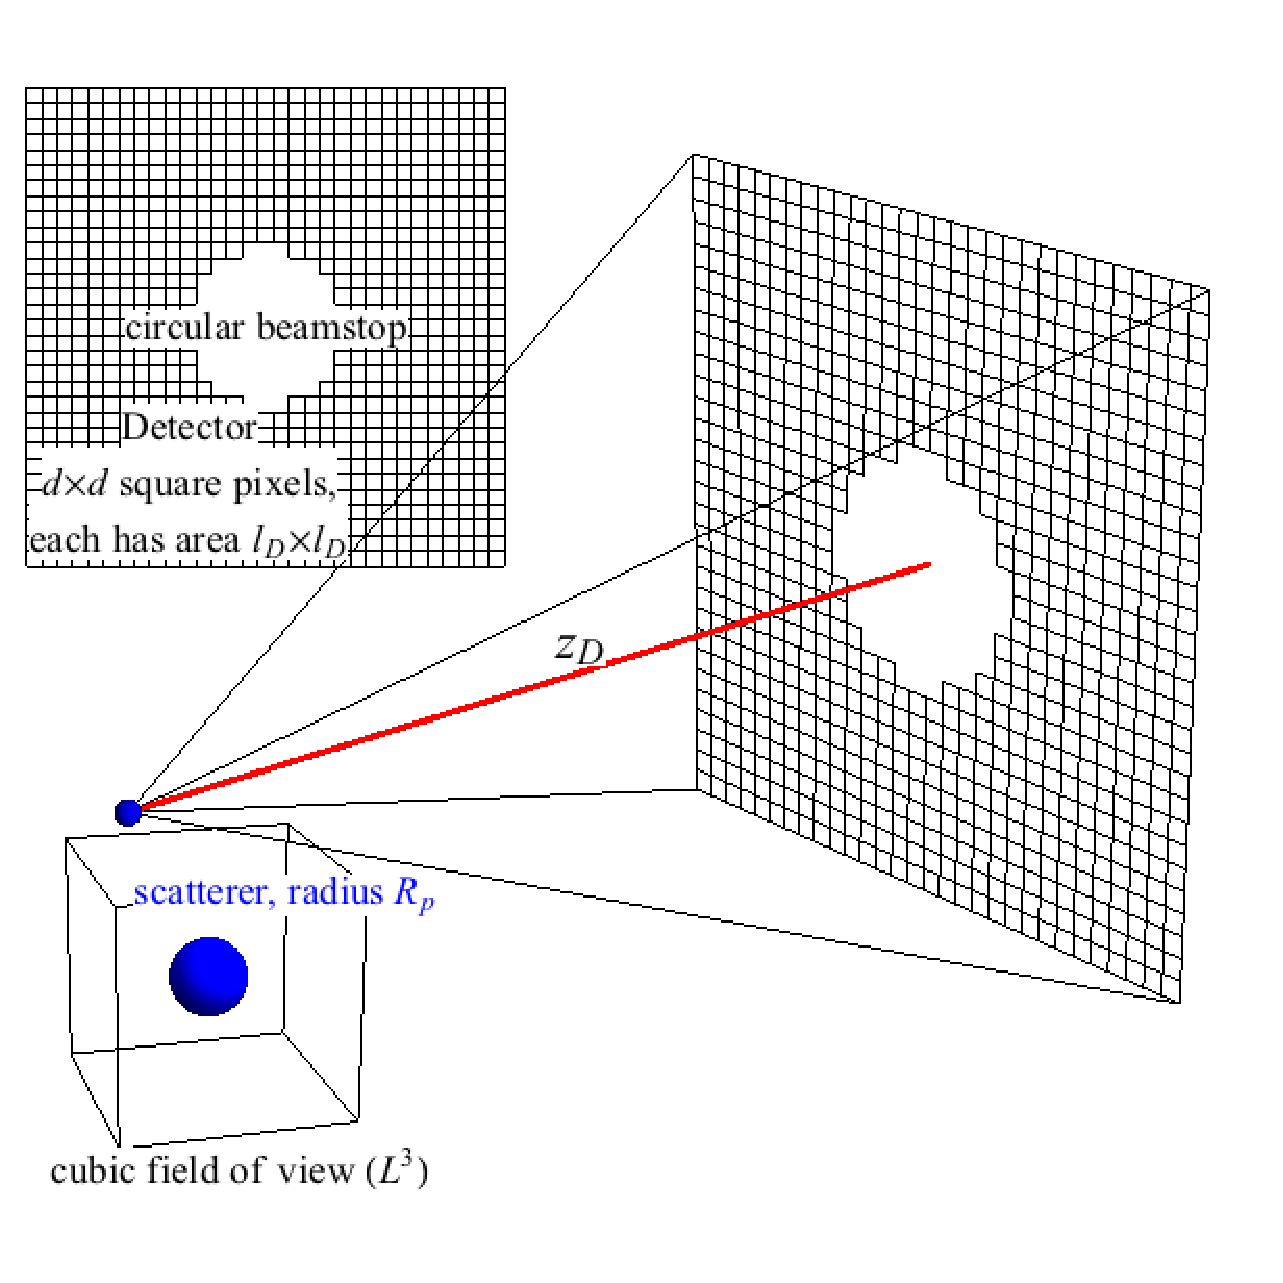
\includegraphics{figures/geometry.eps}
%\end{figure}


\end{document}                    % DO NOT DELETE THIS LINE
%%%%%%%%%%%%%%%%%%%%%%%%%%%%%%%%%%%%%%%%%%%%%%%%%%%%%%%%%%%%%%%%%%%%%%%%%%%%%%
